
\section{Results}

The model has been applied to the protocol of the k-armed bandit task described in the methods section.


% ------- stationary ------- %

\subsection{Stationary environment}
In the first part, the reward distribution is stationary, and the agent evaluated against the chance and the optimal strategy in the measure of \textit{regret}.


\begin{figure}[ht]
    \centering
    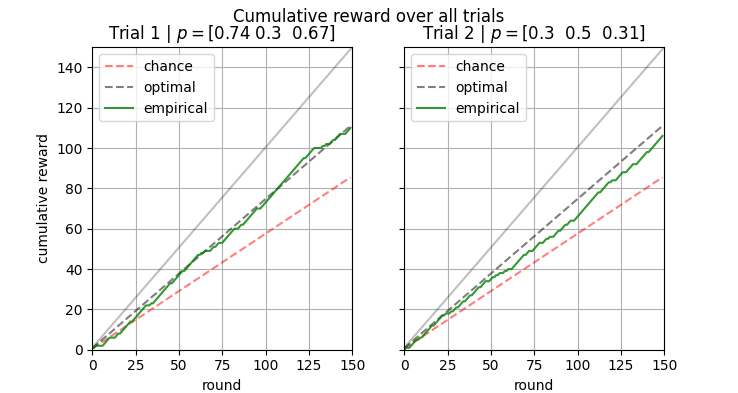
\includegraphics[width=0.8\textwidth]{figures/hsnn_results_trials_1.png}
    \caption{\textsc{Cumulative reward over trials - }\textit{For each round: the dashed line represents the maximum cumulative reward obtainable by receiving 1 at each round; the black solid line represents the expected cumulative reward for the greediest strategy, i.e. always choosing the arm with the
    highest expected reward; the green solid line represents the cumulative reward obtained by the agent; in red the expected cumuluative reward obtained by a random agent.}}
    \label{fig:results_trials_1}
\end{figure}

\begin{figure}[ht]
    \centering
    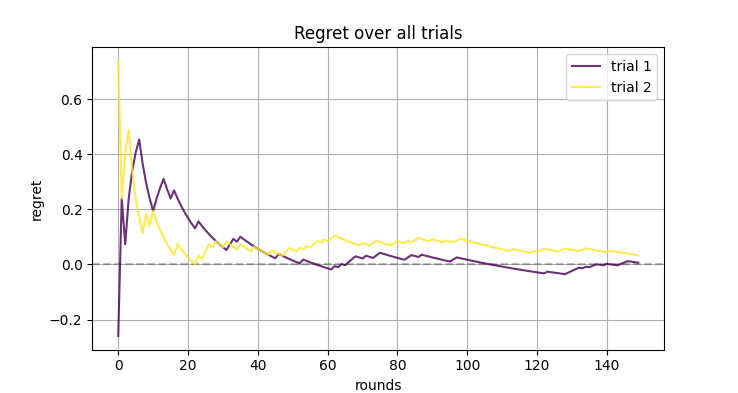
\includegraphics[width=0.8\textwidth]{figures/hsnn_results_regret_1.png}
    \caption{\textsc{Regret over rounds for each trial - }\textit{Each line represents the cumulative regret normalized by number of rounds.}}
    \label{fig:results_regret_1}
\end{figure}


\begin{figure}[ht]
    \centering
    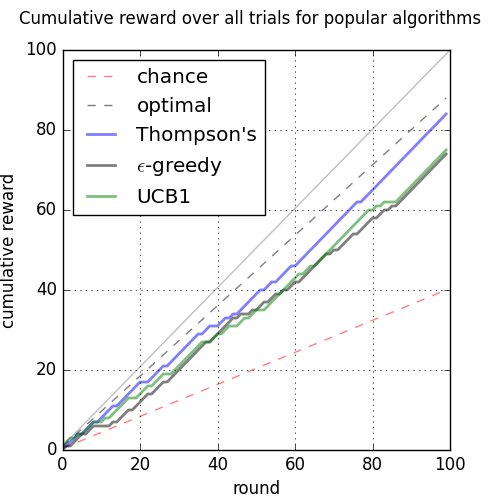
\includegraphics[width=0.4\textwidth]{figures/lit_models_.png}
    \caption{\textsc{Performance of known algorithms - }\textit{Comparison of various models taked from the literature.}}
    \label{fig.lit_models_1}
\end{figure}

% ------- non-stationary ------- %

\subsection{Non-stationary environment}
In the second part, the reward distribution is non-stationary, the agent performance is evaluated as before, but with the focus on the recovery speed following the change in the distribution.


\begin{figure}[ht]
    \centering
    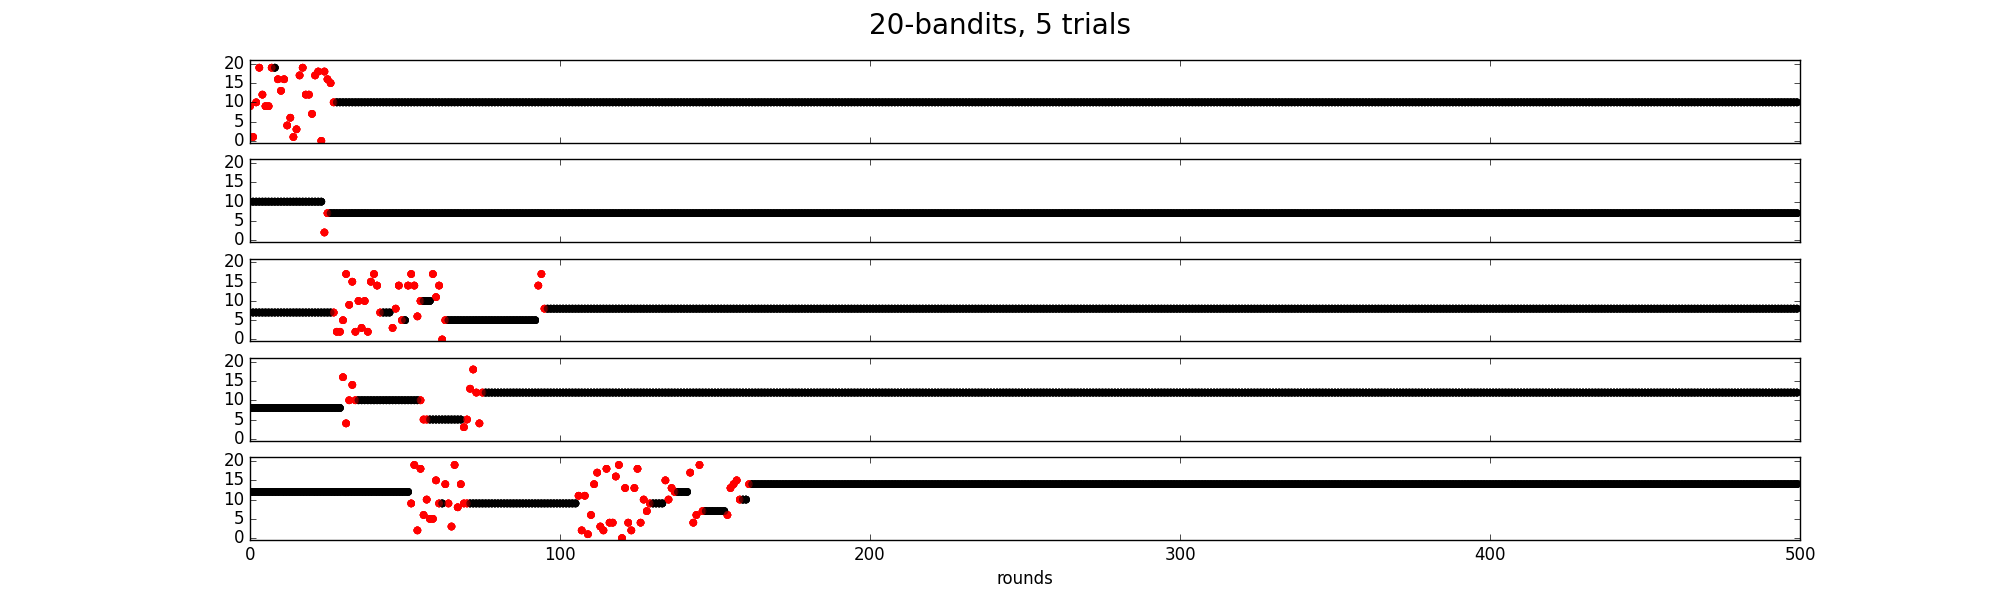
\includegraphics[width=0.8\textwidth]{figures/minmod_a.png}
    \caption{\textsc{Option selected over rounds for each trial}\\\textit{The red dots are choices made randomly, the black dots are intentional selections}}
    \label{fig:results_minmod_a}
\end{figure}



% ------- policy ------- %

\subsection{Policy}

% - policy as probability distribution - %
The agent's policy is described in terms of the probability of choosing each arm, and the evolution of the policy is shown in the stationary and non-stationary environment.


\hfill \break
% - policy as neural activity - %
The agent's policy is also described in terms of the neural activity, and the evolution of the policy is shown in the stationary and non-stationary environment.



